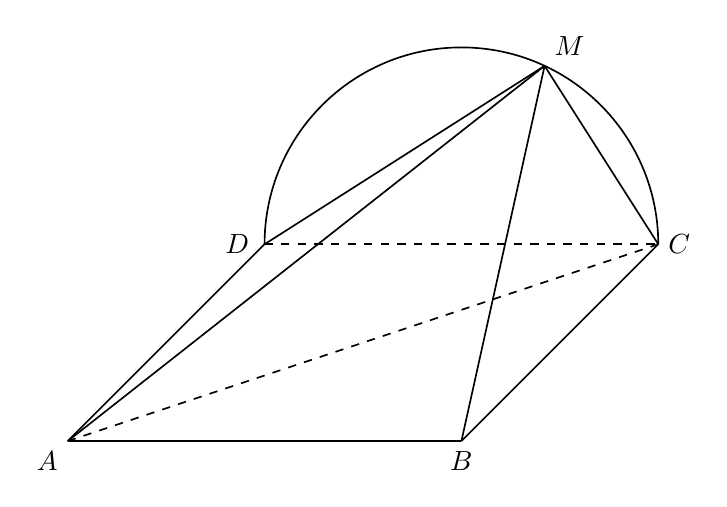
\begin{tikzpicture}[line width=0.6pt, font=\normalsize]
  \coordinate (D) at (0,1);
  \coordinate (C) at (5,1);
  \coordinate (A) at (-2.5,-1.5);
  \coordinate (B) at (2.5,-1.5);
  \coordinate (M) at (3.556545654,3.265769468);
  % True semicircle with diameter DC
  \draw (D) arc[start angle=180, end angle=0, x radius=2.5, y radius=2.5];
  \draw[dashed] (D) -- (C);
  \draw (A) -- (B);
  \draw (B) -- (C);
  \draw (A) -- (D);
  \draw (A) -- (M);
  \draw (D) -- (M);
  \draw (M) -- (B);
  \draw (M) -- (C);
  % Diagonal AC is dashed in the science figure
  \draw[dashed] (A) -- (C);
  \node[below left] at (A) {$A$};
  \node[below] at (B) {$B$};
  \node[right] at (C) {$C$};
  \node[left,xshift=-2.00bp,yshift=0.00bp] at (D) {$D$};
  \node[above right] at (M) {$M$};
\end{tikzpicture}
